\documentclass[a4paper, 10pt]{article}
\usepackage[english]{babel}
\usepackage[utf8]{inputenc}
\usepackage{amsfonts}
\usepackage{amsmath}
\usepackage{graphicx}
\usepackage{subcaption}
\usepackage[hidelinks]{hyperref}

\author{Maarten de Jonge}
\title{Projective Geometric Algebra}

\begin{document}
\newcommand{\rp}{$\mathbb{R}^{3,3}$ }

\begin{center}

\vspace{2.5cm}

% [CHANGE] The title of your thesis. If your thesis has a subtitle, then this
% should appear right below the main title, in a smaller font.
\begin{Huge}
Projective Geometric Algebra
\end{Huge}

\vspace{1.5cm}

% [CHANGE] Your full name. In case of multiple names, you can include their
% initials as well, e.g. "Jan G.J. van der Wegge".
Maarten de Jonge \\
% [CHANGE] Your student ID, as this has been assigned to you by the UvA
% administration.

\vspace{1.5cm}

% [DO NOT CHANGE]
Bachelor thesis\\
% [CHANGE] Whether your Bachelor thesis is 6 ECTS (regular) or 9 ECTS (Honours
% programme).
Credits: 18 EC

\vspace{0.5cm}

% [DO NOT CHANGE] The name of the educational programme.
Bachelor Opleiding Kunstmatige Intelligentie

\vspace{0.25cm}

% [DO NOT CHANGE] The addess of the educational programme.
University of Amsterdam\\
Faculty of Science\\
Science Park 904\\
1098 XH Amsterdam

\vspace{4cm}

\emph{Supervisor}\\
% [CHANGE] The name of your supervisor. Include the titles of your supervisor,
% as well as the initials for *all* of his/her first names.
Dr. ir. Leo Dorst

\vspace{0.25cm}

% [CHANGE] The address of the institute at which your supervisor is working.
% Be sure to include (1) institute (is appropriate), (2) faculty (if
% appropriate), (3) organisation name, (4) organisation address (2 lines).
Intelligent Systems Laboratory Amsterdam \\
Informatics Institute \\
Faculty of Science\\
University of Amsterdam\\
Science Park 904\\
1098 XH  Amsterdam

\vspace{1.5cm}

% [CHANGE] The date at which you will finalize and submit your thesis.
\today

\end{center}
\clearpage

\tableofcontents
\clearpage

\section{Introduction}
This introduction gives a short introduction to various concepts essential to
the research, mainly projective geometry and geometric algebra. Subsequently,
these are tied together and the topic of this research emerges.

\subsection{Projective Geometry}
Projective geometry is the study of geometric properties invariant under
projective transformations, with applications in areas such as computer vision,
computer graphics, and quantum physics. Compared to the familiar Euclidean
geometry, the space is extended with elements at infinity. This solves a number
of irregularities and adds a greater expressive power to the algebra. For
example, two different lines in the same plane in Euclidean geometry have either
one or zero (when the lines are parallel) points of intersection. With the
addition of points at infinity, this becomes more general: two different lines
in the same plane always have one point of intersection, where parallel lines
will meet in infinity. This mimics observations in real life, e.g. train tracks
which appear to converge as the distance increases, eventually
appearing to meet at an infinite distance even though they are obviously parallel.
An important advantage of this is in software implementation: you will not have
to check for edge cases when there are no edge cases, leading to both simpler
and more efficient implementations.

\subsection{Geometric Algebra}
Geometric algebra\cite{dorst2009geometric} is an algebra over an $n$-dimensional
vector space, similar to
linear algebra. Unlike linear algebra however, geometric algebra allows for
coordinate-free transformations in a structure-preserving manner by using the
geometric product. Of further importance is the outer product, which constructs
higher-dimensional subspaces from basic elements. Of the various models of
geometric algebra in use, the homogenous model is of most interest for this thesis.
This model embeds $n$-dimensional space in a $n + 1$-dimensional representational
space (similarly to the homogenous model of linear algebra).  Lines are
represented as the outer product of two vectors (which themselves represent
points); this is referred to as a \emph{2-blade} or more generally a
\emph{bivector}. These line elements can be represented as vectors on a basis of
$n \choose 2$ bivectors (the amount of unique bivectors in $n$-dimensional
space), leading to a space which uses lines as its basis elements (a \emph{line
space}). Applying this to lines in homogeneous 3D space leads to an equivalence
with Pl\"{u}cker coordinates, a system for representing 3D lines by means of 6
homogeneous coordinates. This leads to a system referred to as the Pl\"{u}cker
model of geometric algebra. These models are further explored in section
\ref{sec:background}.

\subsection{Research Topic}
Recent research of the Pl\"{u}cker model (done by \cite{hangbo2011}
\cite{dorst2013versors} \cite{pottmann2001computational} \cite{dekok2012} as
elaborated on in section 2) has provided the geometric elements of the space
with visual interpretations. GAViewer, a geometric algebra visualisation tool
which currently has partial support for the Pl\"{u}cker model, will be extended
with a particularly troublesome to implement 3-blade whose visualisation is in
the form of a regulus (figure \ref{fig:regulus}).

In addition, the Pl\"{u}cker model can be applied to 2D projective geometry by
taking a cross-section of a regulus to be a conic section in 2D and considering
only transformations which keep this cross-section constant. 
As an illustration, the testing for membership of a point to a conic section
will be explored.

\begin{figure}[htbp]
  \centering
  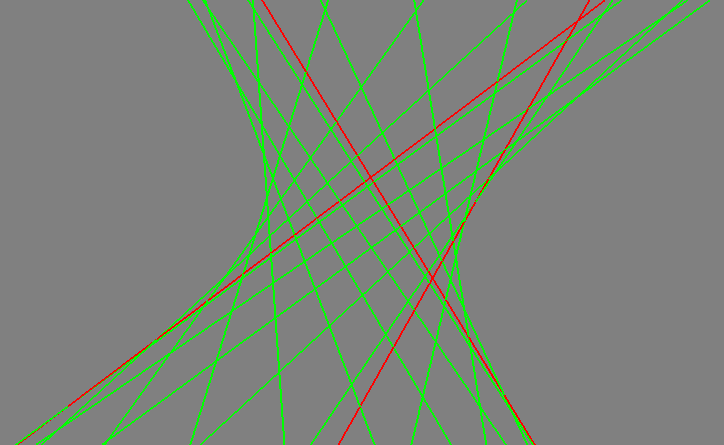
\includegraphics[width=0.5\textwidth]{regulus.png}
  \caption{A regulus}
  \label{fig:regulus}
\end{figure}

\section{Literature Review}
Li and Zhang\cite{hangbo2011} model line geometry in a 6D space, representing
lines by means of their Pl\"{u}cker coordinates (with the constraint that the
vector must square to zero, i.e. be a null vector).  The 6D vector of a line's
Pl\"{u}cker coordinates corresponds to the coordinates of of the line's
direction and moment on a basis of 2-blades in $\wedge^2(V^4)$, a bivector space
over the 4D homogeneous vector space. Through a clever correspondence with the
homogeneous space, Li and Zhang also provide a metric for the 6D
representational space and show that it has the signature $\mathbb{R}^{3, 3}$. They
proceed to give geometric interpretations of the various blades that can be
formed in $\mathbb{R}^{3, 3}$.

Pottmann and Wallner\cite{pottmann2001computational} do similarly, except they
stay within the domain of linear algebra, giving a different viewpoint to what is
essentially the same geometry.

Leo Dorst\cite{dorst2013versors} provides visual representations for many of the
geometric features described by \cite{hangbo2011} and
\cite{pottmann2001computational} and describes how to extract the data required
for implementing these visualizations in software. Additionally, the paper
contains a novel approach to modeling 2D projective geometry in the previously
described \rp, defining the elementary operations (translations, scaling,
perspective transformations, a rotation and a squeeze) in terms of their
transformation matrices.

GAViewer\footnote{\url{http://www.geometricalgebra.net/gaviewer\_download.html}}
is a graphical calculator for geometric algebra which handles many different
algebraic models. Patrick de Kok\cite{dekok2012} implemented the
Pl\"{u}cker model of Li and Zhang in GAViewer and added many of the
visualizations described by Dorst.

Cinderella\cite{richter1999interactive} is a software package for performing
interactive 2D projective geometry using a 6D homogeneous representation with
complex numbers. This avoids the edge cases commonly experienced in classic
Euclidean geometry. For a good read on their approach to this problem, see
\url{http://doc.cinderella.de/tiki-index.php?page=Theoretical+Background}.
Note that their use of 6 dimensions to represent 2D geometry hints at a
correspondence with the model described by Dorst, who also uses 6 (albeit
different) dimensions for representing 2D projective geometry.

\section{Theoretic Background}
\label{sec:background}

\subsection{The Homogeneous Model}
The homogeneous model of geometric algebra works similarly to the equally named
model of linear algebra; an $n$D space is embedded in an $n+1$D representational
space, allowing for elements to be represented offset from the origin. Due to
the focus of this thesis, the focus will specifically be on the embedding of
$\mathbb{R}^3$ in the 4-dimensional vector space $V^4$ (defining a metric for
this space is not necessary).

In the homogeneous model, the basis ${e_1, e^2, e^3}$ is extended by an
additional element $e_0$. This origin of $\mathbb{R}^3$ is taken to be offset by
a distance of 1 in the $e_0$ direction. As in linear algebra, elements that have
a non-zero $e_0$ component are interpreted by projecting them onto
$\mathbb{R}^3$: if the component is not 1, the entire element is rescaled such
that the $e_0$ component does become 1.

In this model, vectors are interpreted as points. The point $\mathbf{p}$ in
$\mathbb{R}^3$ is represented as $e_0 + \mathbf{p}$. Elements without an $e_0$
component are located entirely outside of $\mathbb{R}^3$ and are considered
points at infinity or directions. Points with an $e_0$ component will be
referred to as \emph{finite points}, in contrast to the infinite points or
directions without an $e_0$ component.

\subsubsection{Lines}
Of specific interest to this thesis are lines. In the homogeneous space, lines
are formed by the outer product of two points, be they finite or infinite.
There are 3 methods of constructing a line:
\begin{itemize}
  \item The outer product of two finite points constructs the line through
    both points
  \item The outer product of a point $p$ and a direction $d$ (a finite and infinite
    point) constructs the line through $p$ with the direction $d$.
  \item Two infinite points represent the direction of the line and the dual of
    the line's moment, the plane that goes through the line and the origin.
    Their outer product also produces the corresponding line.
\end{itemize}
Two of these methods are shown in figure \ref{fig:lines}.

\begin{figure}
  \centering
  \begin{subfigure}[b]{0.5\textwidth}
    \centering
    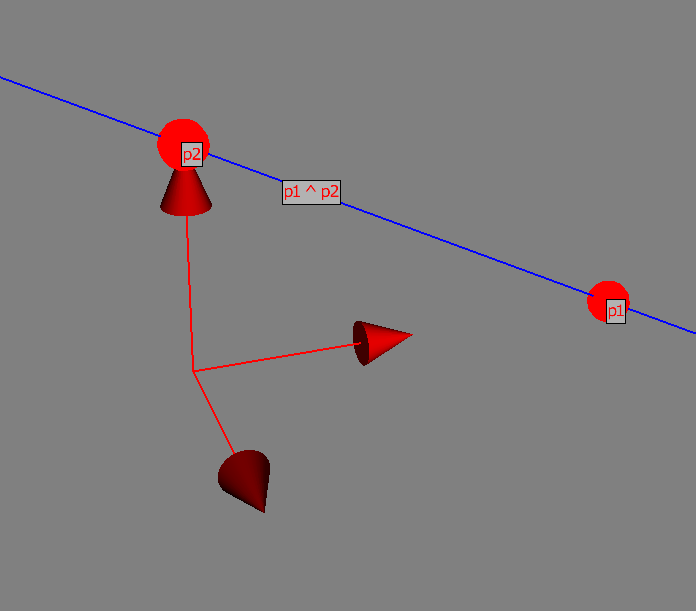
\includegraphics[width=\textwidth]{./points.png}
    \caption{Two points}
    \label{fig:points}
  \end{subfigure}%
  ~ % spacing
  \begin{subfigure}[b]{0.5\textwidth}
    \centering
    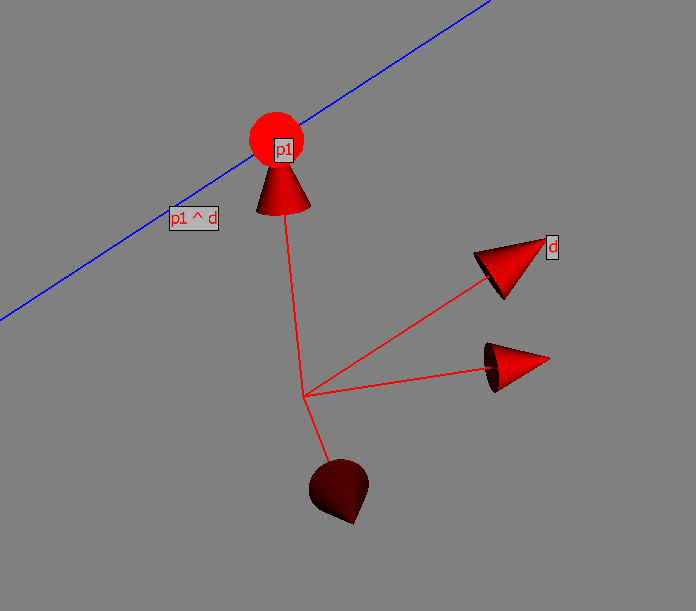
\includegraphics[width=\textwidth]{point_dir.png}
    \caption{A point and a direction}
    \label{fig:point_dir}
  \end{subfigure}
  \caption{Two of the ways of constructing a line}
  \label{fig:lines}
\end{figure}

\subsection{Pl\"{u}cker Space}
Lines in $V^4$ can be decomposed onto a basis of bivectors (bold elements refer
to elements described entirely in the embedded $\mathbb{R}^3$):
\begin{align*}
   p \wedge q &= (e_0 + \mathbf{p}) \wedge (e_0 + \mathbf{q}) = (e_0 \wedge \mathbf{q}) + (\mathbf{p} \wedge e_0) + (\mathbf{p} \wedge \mathbf{q}) \\
         &= (e_0 \wedge \mathbf{q}) + (e_0 \wedge - \mathbf{p}) + \mathbf{p} \wedge \mathbf{q} \\
         &= e_0 \wedge (\mathbf{q} - \mathbf{p}) + \mathbf{p} \wedge \mathbf{q} \\
         &= (\mathbf{p} - \mathbf{q}) e_0 + (\mathbf{p} \times \mathbf{q}) I_3 \\
         &= \alpha e_1 e_0 + \beta e_2 e_0 + \gamma e_3 e_0 + \delta e_1 I_3 +
         \epsilon e_2 I_3 + \zeta e_3 I_3 \\
         &= \alpha e_1 e_0 + \beta e_2 e_0 + \gamma e_3 e_0 + \delta e_2 e_3 +
         \epsilon e_3 e_1 + \zeta e_1 e_2
\end{align*}
These coefficients define a line on a basis of bivectors in $V^4$, and
correspond directly to the Pl\"{u}cker coordinate description of a line by means
of its direction and moment. This leads to a bivector space $\wedge^2 V^4$ with
the basis ${e_{01}, e_{02}, e_{03}, e_{23}, e_{31}, e_{12}}$. Note that not
every element on this basis represents a line; lines have the requirement that
their the dot product between its direction and moment must be zero. This is
captured in the Grassmann-Pl\"{u}cker condition:
\begin{align*}
  l_{01} l_{23} + l_{02} l_{31} + l_{03} l_{12} = 0
\end{align*}
where $l_{ij}$ are the coefficients of the bivector basis.

An embedding from from $V^4$ to $\wedge^2 V^4$ is easily defined:
\begin{align*}
Em(A) =
\begin{cases}
  e_{ij} & \text{if } A = e_i \wedge e_j \\
  Em(B) + Em(C) & \text{if } A = B + C \\
  Em(B) \wedge Em(C) & \text{if } A = B \wedge C \\
  Em(B) \rfloor Em(C) & \text{if } A = B \rfloor C
\end{cases}
\end{align*}

The metric for this space is given by \cite{hangbo2011}. Given two bivectors $A$
and $B$ in $V^4$ and their embeddings in $\wedge^2 V^4$ $Em(A)$ and $Em(B)$, the
inner product is defined as:
\begin{align*}
  Em(A) \cdot Em(B) = [A ^ B]
\end{align*}
where the bracket operator refers to proportionality with the pseudoscalar $I_4$
of $V^4$. This leads to the multiplication table show in table \ref{table:mult}.
\begin{table}
  \centering
  \begin{tabular}{|c | c c c | c c c|}
    \hline
    & $e_{01}$ & $e_{02}$ & $e_{03}$ & $e_{23}$ & $e_{31}$ & $e_{12}$ \\
    \hline
    $e_{01}$ & 0 & 0 & 0 & 1 & 0 & 0 \\
    $e_{02}$ & 0 & 0 & 0 & 0 & 1 & 0 \\
    $e_{03}$ & 0 & 0 & 0 & 0 & 0 & 1 \\
    \hline
    $e_{23}$ & 1 & 0 & 0 & 0 & 0 & 0 \\
    $e_{31}$ & 0 & 1 & 0 & 0 & 0 & 0 \\
    $e_{12}$ & 0 & 0 & 1 & 0 & 0 & 0 \\
    \hline
  \end{tabular}
  \caption{}
  \label{table:mult}
\end{table}

This table can be used to implement the inner product:
\begin{align*}
  a \cdot b = a^T M b 
\end{align*}
where
\begin{align*}
  M =
  \begin{bmatrix}
    0 & 0 & 0 & 1 & 0 & 0 \\
    0 & 0 & 0 & 0 & 1 & 0 \\
    0 & 0 & 0 & 0 & 0 & 1 \\
    1 & 0 & 0 & 0 & 0 & 0 \\
    0 & 1 & 0 & 0 & 0 & 0 \\
    0 & 0 & 1 & 0 & 0 & 0 \\
  \end{bmatrix}
\end{align*}
and $M$ is referred to as the metric matrix of this basis. Diagonalising the
metric matrix leads to a basis of
\begin{align*}
  \lbrace a_+, b_+, c_+, a_-, b_-, c_- \rbrace =
  \lbrace \frac{ e_{01} + e_{23} }{\sqrt{2}}, \frac{ e_{02} + e_{31} }{\sqrt{2}}, \frac{ e_{03} + e_{12} }{\sqrt{2}}, 
  \frac{ e_{01} - e_{23} }{\sqrt{2}}, \frac{ e_{02} - e_{31} }{\sqrt{2}}, \frac{
    e_{03} - e_{12} }{\sqrt{2}} \rbrace
\end{align*}
with a corresponding metric matrix
\begin{align*}
  M =
  \begin{bmatrix}
    1 & 0 & 0 & 0 & 0 & 0 \\
    0 & 1 & 0 & 0 & 0 & 0 \\
    0 & 0 & 1 & 0 & 0 & 0 \\
    0 & 0 & 0 & -1 & 0 & 0 \\
    0 & 0 & 0 & 0 & -1 & 0 \\
    0 & 0 & 0 & 0 & 0 & -1 \\
  \end{bmatrix}
\end{align*}

This shows that the space has a metric of \rp.
To disambiguate between these two different axes, the first one will be referred
to as the \emph{null basis} (because its basis vectors square to zero), while the
second one is the \emph{unit basis}.

Interpretations of the graded elements of this space are given by
\cite{dekok2012}, \cite{hangbo2011} and \cite{dorst2013versors}. The next
section will focus on the regulus, a 3-blade formed from three skew lines. It is
a collection of an infinite amount of skew lines which all intersect each of the
three lines that construct the regulus, as shown in figure 1 (the red lines were
used to constract the regulus).

\subsection{Regulus Parameters}
The regulus can be described by three axes; The main axis describes the
orientation of the regulus, while two additional axes represent the major and
minor axes of the ellipse at the center cross-section.

\begin{figure}[htbp]
  \centering
  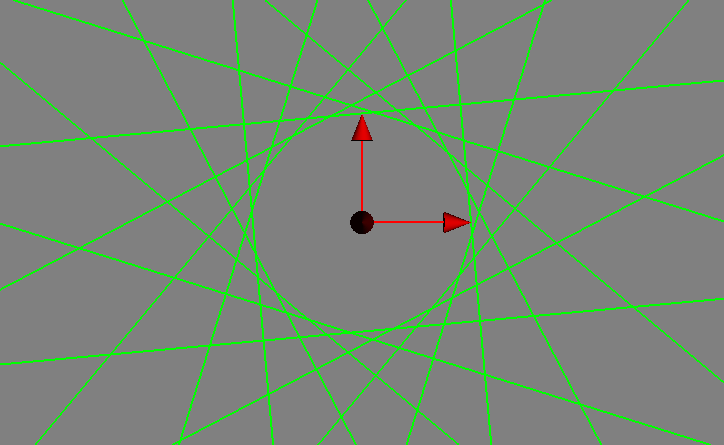
\includegraphics[width=0.5\textwidth]{axes.png}
  \caption{The standard regulus with its axes shown in red. The camera is
    oriented along the main axis.}
  \label{fig:axes}
\end{figure}

The standard regulus $R_0$ is formed by the outer product of the following three
skew lines:
\begin{itemize}
  \item $e_{02} + e_{12} + e_{03} - e_{31} / \sqrt(2)$
  \item $-e_{01} + e_{12} + e_{03} - e_{23} / \sqrt(2)$
  \item $-e_{02} + e_{12} + e_{03} + e_{31} / \sqrt(2)$
\end{itemize}

This is not a unique factorisation however; the resulting 3-blade could also be
factorised as $(e_{01} - e_{23}) ^ (e_{02} - e_{31}) ^ (e_{03} - e_{12})$, which
equates to the factors $a_-, b_-$ and $c_+$ of the unit basis. This
orthogonal factorisation corresponds to the axes of the regulus; the lines of
the axes can be retrieved by addition with their associate vectors, i.e.:
\begin{align*}
  a_+ + a_- = e_{01} \\
  b_+ + b_- = e_{02} \\
  c_+ + c_- = e_{03}
\end{align*}
The associate vectors themselves correspond to the axes of the dual standard
regulus $R_{0}^*$. These factors will remain orthogonal after the standard
regulus gets transformed to an arbitrary regulus by means of a conformal
transformation\footnote{A conformal transformation is a transformation which
  preserves angles}.
The lines of $R_{0}$ slope at an angle of $\pi / 4$ relative to its cross
section.

Because there is no reliable way of obtaining such a factorisation, a different
approach has to be taken. One might note that the factors corresponding to the
axes commute with the regulus, while their associate anticommutes:
\begin{align*}
  a_- R_0 &= a_- \rfloor R_0 + a_- \wedge R_0 = a_- \rfloor R_0 =  R_0 \lfloor a_- = R_0 a_- \\
  a_+ R_0 &= a_+ \rfloor R_0 + a_+ \wedge R_0 = a_+ \wedge R_0 = -R_0 \wedge a_+ = -R_0 a_+ \\
\end{align*}

These properties can be easily described by means of a linear operator
\underline{R} based on the regulus R\cite{dorst2013versors}:
\begin{align*}
  \underline{R} : x \mapsto R^{-1} x R
\end{align*}
It is easy to prove that that commutation and anti-commutation properties are
captured by the eigenvectors of eigenvalues 1 and -1 respectively.
For eigenvalue 1:
\begin{align*}
  R^{-1} x R &= x \\
  x R &= R x
\end{align*}
and similarly for eigenvalue -1:
\begin{align*}
  R^{-1} x R &= -x \\
  x R &= R (-x)
\end{align*}

This means that the axes can be retrieved from the eigenvectors of eigenvalue 1 of
the operator \underline{R} along with their associates of eigenvalue -1. Recall
that the axes of $R_0$ correspond to $a_-$, $b_-$ and $c_+$; two of them square
to the same sign, while one squares to the opposite sign. The one with the
differing sign corresponds to the main axis. This property remains intact
after a conformal transformation from $R_0$ to a general regulus $R$.

The length of the axes also follows naturally from this process. Given an
scaling factor $e^\gamma$, the finite components of the eigenvectors scales with
a factor $e^\gamma$ while the infinite components scale with
$e^{-\gamma}$\cite{dorst2013versors}. This
means that the eigenvectors can be freely rescaled without losing any
information about the axes' lengths.

With this knowledge, the algorithm for obtaining a regulus' axes is as follows:
\begin{enumerate}
  \item Obtain eigenvectors of the linear operator $\underline{R}$
  \item Look for the two eigenvectors of eigenvalue 1 whose squares have the
    same sign; these denote the center ellipse, while the other one denotes the
    main axis.
  \item Add these vectors to their associate eigenvectors of eigenvalue -1 to
    obtain the lines of the axes.
\end{enumerate}

\subsection{2D geometry}
When looking at the regulus straight from its main axis, it appears to form an
ellipse, defined by its tangents (figure \ref{fig:circle}). Since vectors in the
Pl\"{u}cker space represent lines, some way of representing points must be
devised. In particular, points that reside in a particular plane. This is easily
done by means of line pencils; the outer product of two intersecting lines
represents the collection of coplanar lines going through that point (figure
\ref{fig:pencil}, visualization implemented by \cite{dekok2012}).

\begin{figure}[htbp]
  \centering
  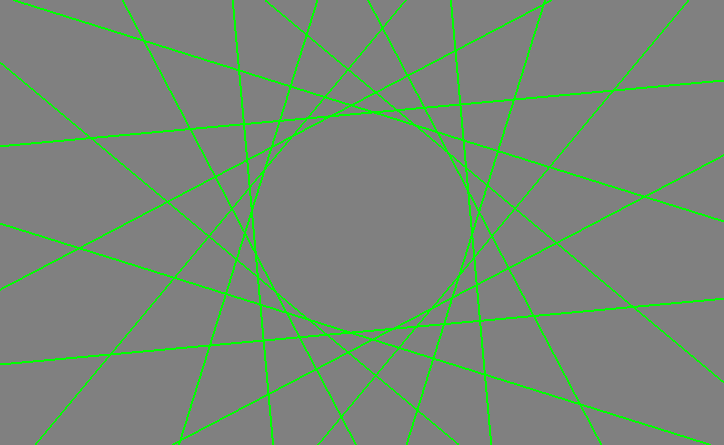
\includegraphics[width=0.7\textwidth]{circle.png}
  \caption{A circle as represented by the cross section of the standard regulus.}
  \label{fig:circle}
\end{figure}

\begin{figure}[htbp]
  \centering
  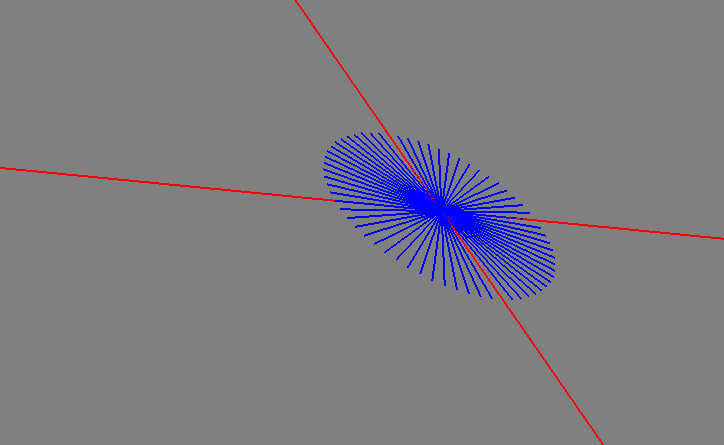
\includegraphics[width=0.7\textwidth]{pencil.png}
  \caption{A pencil of lines}
  \label{fig:pencil}
\end{figure}

\section{Implementation}
\subsection{Eigenvectors}
Following the algorithm described in the previous section, the first step is to
obtain the eigenvectors of a linear operator. There is no geometric process for
this, so the obvious thing to do is to convert the transformation to a
transformation matrix and use common techniques from linear algebra to do the
eigenvector decomposition. 

The transformation matrix $F$ will be defined by means of its elements $F(i, j)$
where $i$ refers to the row and $j$ to the column. The transformation performed
by the linear operator on a vector $x$ is referred to as $f[x]$. Additionally,
$b_i$ refers to the i'th basis vector while $b^i$ refers to the reciprocal of
the i'th basis vectors (that is, $b_i \cdot b^j = 1$):
\begin{align}
  F(j, i) = f[b_i] \cdot b^j \label{eq:matrix}
\end{align}
This algorithm is taken from \cite{dorst2009geometric}. Keep in mind that in
this case, the inner product is taken in the Pl\"{u}cker space, which is
important because of the non-Euclidean metric. For simplicity and consistency with earlier
work, all calculations are implemented on the null basis. The basis vectors are
6D vectors whose components are coefficients on the ${e_{01}, e_{02}, e_{03},
  e_{23}, e_{31}, e_{12}}$ basis, e.g. the vector $\begin{bmatrix} 1 & 0 & 1 & 0
  & 0 & 0 \end{bmatrix}$ represents the geometric element $e_{01} + e_{03}$.

Formula \ref{eq:matrix} can be simplified by observing a number of properties:
\begin{itemize}
  \item $x \cdot y$ can be written as $x^T M y$, where $M$ is the metric matrix
    for the null basis
  \item The metric matrix squares to the identity matrix (i.e. $M * M = I$)
  \item As long as a metric matrix contains only the values -1, 0 and 1, it acts
    as a selection operation for a basis vector's reciprocal; if $b_{1}^{T} (M b_{2}) = 1$
    then $(M b_{2})$ must be the reciprocal of $b_{1}$.
\end{itemize}
This allows for simplification of the previous formula:
\begin{align*}
  F(j, i) &= f[b_i] \cdot b^j \\
  F(j, i) &= f[b_i]^T M b^j \\
  F(j, i) &= f[b_i]^T M (M b_j) \\
  F(j, i) &= f[b_i]^T (M M) b_j \\
  F(j, i) &= f[b_i]^T b_j
\end{align*}
The transformation $f[b_i]$ is realized by converting the vector $b_i$ to it's
corresponding geometrical element, applying the regulus operator to it and
converting the result back to a vector representation.

Once the transformation matrix has been constructed, the eigenvectors can be
found by any of the conventional methods. I opted for the
Eigen\footnote{http://eigen.tuxfamily.org/} library for C++.

\subsection{Matching associates}
The obtained eigenvectors will likely not be in a usable state yet; any scalar
multiple of an eigenvector is also an eigenvector, and different norms make it
hard to match associates, which are supposed to exactly cancel out the infinite
components. This is easily alleviated in two ways. First, the eigenvectors are
rescaled such that they square to 1. This solves part of the problem, but still
leaves potential inconsistencies in minus signs. For example, when looking at
the element $(e_{01} - e_{23}) / \sqrt{2})$ and its associate $(e_{01} + e_{23})
/ \sqrt{2})$, the associate might end up being in the form of $-e_{01} - e_{23})
/ \sqrt(2)$; the element would still square to 1, but adding the elements would
produce an infinite line rather than a finite one as desired.
This problem is fixed by making sure that the first finite component of each
eigenvector has a positive coefficient; vectors that do not meet this demand
shall be multiplied by $-1$ until they do.

Once the eigenvectors have been coaxed into a usable form, finding the
associates is a matter of a trivial brute-force search. For each of the three
eigenvectors of value 1, each eigenvector valued $-1$ is checked so see if their
sum produces a finite line. After this process, each eigenvector will have an
associate and the axis lines are now known from their sum.

\subsection{Slant}
An additional parameter of the regulus is the slant of its lines, which is the
direction the lines rotate along the regulus' center ellipse (more on this in
the next section). The slant follows from the squares of the eigenvectors of
eigenvalue 1: two negatively squared eigenvectors correspond to the orientation
of the standard regulus, while two positively squared eigenvectors correspond to
the dual standard regulus' orientation.

\subsection{Drawing}
Drawing of the regulus in GAViewer (which uses OpenGL for its drawing) is done
by normalising the two axes perpendicular to the main axis such that they span a
circle. Along certain intervals of the circle, a line will be drawn with the
correct scaling applied.  This is done by scaling the OpenGL modelview matrix
appropriately with the weights obtained from the axes and drawing the lines
sloping at $\pi / 4$.

\section{Results}
The regulus visualization is implemented in the GAViewer software and should
allow for arbitrary transformations to be drawn correctly. Figure
\ref{fig:reguli} shows two examples.

\begin{figure}
  \centering
  \begin{subfigure}[b]{0.5\textwidth}
    \centering
    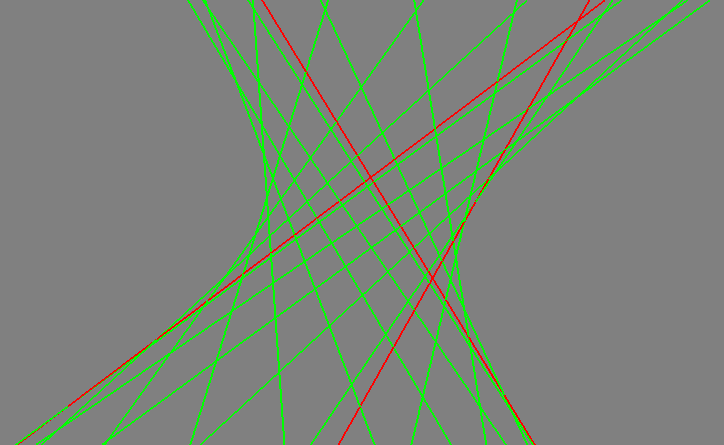
\includegraphics[width=\textwidth]{./regulus.png}
    \caption{Standard regulus, the skew lines that form it shown in red}
  \end{subfigure}%
  ~ % spacing
  \begin{subfigure}[b]{0.5\textwidth}
    \centering
    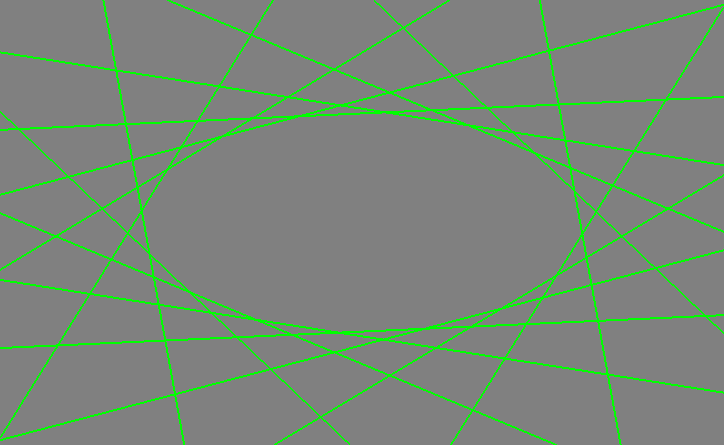
\includegraphics[width=\textwidth]{scaled.png}
    \caption{Scaled by 2 units, top view}
  \end{subfigure}
  \caption{Two examples of reguli}
  \label{fig:reguli}
\end{figure}

A number of bugs remain to be solved however; in particular, translating or
rotating the regulus causes it to be interpreted as a 2-blade (rather than the
3-blade it still is) by the GAViewer software. Fixing this was not possible
within the available timeframe.

Representation of 2D geometry flows naturally from geometry; given a regulus $R$
and a line pencil $P$ coplanar the with cross section of R, $P \rfloor R$ will
result in a grade 1 element. If the center of $P$ intersects any line contained
in the regulus, the result of this contraction will be that finite line. Otherwise, the
result is some not-line. See figure \ref{fig:2d}. As all of the lines of
the reguli intersect the represented conic in the same plane, and $P$ exists in
the same place, this effectively acts like a membership test for a point to the
edge of the conic. If the result of $R \rfloor P$ is a line (i.e. squared to 0),
the point $P$ lies on the conic.

\begin{figure}
  \centering
  \begin{subfigure}[b]{0.5\textwidth}
    \centering
    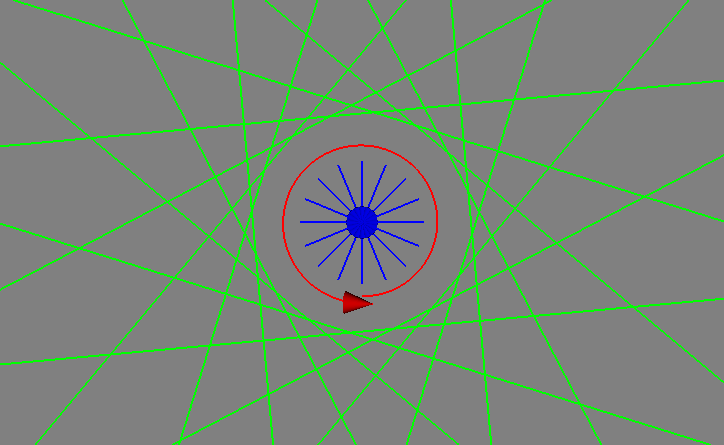
\includegraphics[width=\textwidth]{conic1.png}
  \end{subfigure}%
  ~ % spacing
  \begin{subfigure}[b]{0.5\textwidth}
    \centering
    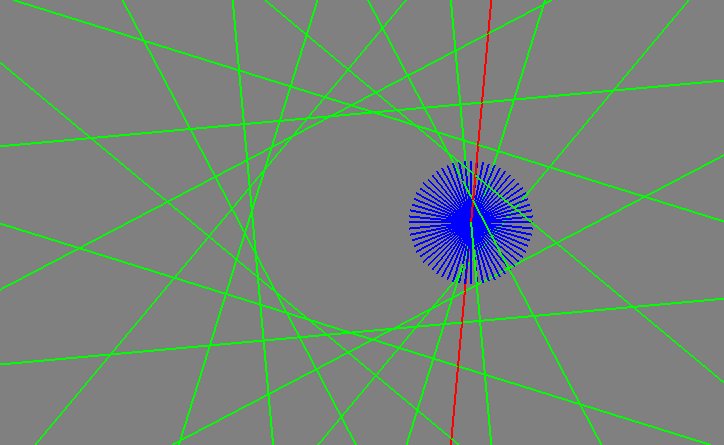
\includegraphics[width=\textwidth]{conic2.png}
  \end{subfigure}
  \caption{Two cases of testing membership of a point (represented by a line
    pencil 2-blade) on a conic (represent by a regulus). Regulus shown in green,
  point in blue and the resulting element in red.}
  \label{fig:2d}
\end{figure}

This knowledge also opens the door for a more intuitive method of drawing a
regulus; as the conic is fully described by the axes, one could move a line
pencil along the conic and use the contraction to directly obtain the lines
contained in the regulus. This has not yet been attempted.

\section{Conclusion}
The regulus can now be succesfully drawn, which opens the door for future
experimentation regarding the Pl\"{u}cker model. Although a few bugs remain,
those should be relatively simple to fix and are purely technical in nature
(rather than algorithmic). The cross section of the regulus appears to be a
promising target for modeling 2D geometry, and representation of points comes
surprisingly easily. Unfortunately, further research in this area was not
possible within the time frame and remains as future work.


\bibliographystyle{plain}
\bibliography{library}
\end{document}
